\documentclass{article} % For LaTeX2e
\usepackage{iclr2024_conference,times}

\usepackage[utf8]{inputenc} % allow utf-8 input
\usepackage[T1]{fontenc}    % use 8-bit T1 fonts
\usepackage{hyperref}       % hyperlinks
\usepackage{url}            % simple URL typesetting
\usepackage{booktabs}       % professional-quality tables
\usepackage{amsfonts}       % blackboard math symbols
\usepackage{nicefrac}       % compact symbols for 1/2, etc.
\usepackage{microtype}      % microtypography
\usepackage{titletoc}

\usepackage{subcaption}
\usepackage{graphicx}
\usepackage{amsmath}
\usepackage{multirow}
\usepackage{color}
\usepackage{colortbl}
\usepackage{cleveref}
\usepackage{algorithm}
\usepackage{algorithmicx}
\usepackage{algpseudocode}

\DeclareMathOperator*{\argmin}{arg\,min}
\DeclareMathOperator*{\argmax}{arg\,max}

\graphicspath{{../}} % To reference your generated figures, see below.
\begin{filecontents}{references.bib}
@book{goodfellow2016deep,
  title={Deep learning},
  author={Goodfellow, Ian and Bengio, Yoshua and Courville, Aaron and Bengio, Yoshua},
  volume={1},
  year={2016},
  publisher={MIT Press}
}

@article{power2022grokking,
  title={Grokking: Generalization beyond overfitting on small algorithmic datasets},
  author={Power, Alethea and Burda, Yuri and Edwards, Harri and Babuschkin, Igor and Misra, Vedant},
  journal={arXiv preprint arXiv:2201.02177},
  year={2022}
}

@article{vaswani2017attention,
  title={Attention is all you need},
  author={Vaswani, Ashish and Shazeer, Noam and Parmar, Niki and Uszkoreit, Jakob and Jones, Llion and Gomez, Aidan N and Kaiser, {\L}ukasz and Polosukhin, Illia},
  journal={Advances in neural information processing systems},
  volume={30},
  year={2017}
}

@article{kingma2014adam,
  title={Adam: A method for stochastic optimization},
  author={Kingma, Diederik P and Ba, Jimmy},
  journal={arXiv preprint arXiv:1412.6980},
  year={2014}
}

@article{ba2016layer,
  title={Layer normalization},
  author={Ba, Jimmy Lei and Kiros, Jamie Ryan and Hinton, Geoffrey E},
  journal={arXiv preprint arXiv:1607.06450},
  year={2016}
}

@article{loshchilov2017adamw,
  title={Decoupled weight decay regularization},
  author={Loshchilov, Ilya and Hutter, Frank},
  journal={arXiv preprint arXiv:1711.05101},
  year={2017}
}

@article{radford2019language,
  title={Language Models are Unsupervised Multitask Learners},
  author={Radford, Alec and Wu, Jeff and Child, Rewon and Luan, David and Amodei, Dario and Sutskever, Ilya},
  year={2019}
}

@article{bahdanau2014neural,
  title={Neural machine translation by jointly learning to align and translate},
  author={Bahdanau, Dzmitry and Cho, Kyunghyun and Bengio, Yoshua},
  journal={arXiv preprint arXiv:1409.0473},
  year={2014}
}

@article{paszke2019pytorch,
  title={Pytorch: An imperative style, high-performance deep learning library},
  author={Paszke, Adam and Gross, Sam and Massa, Francisco and Lerer, Adam and Bradbury, James and Chanan, Gregory and Killeen, Trevor and Lin, Zeming and Gimelshein, Natalia and Antiga, Luca and others},
  journal={Advances in neural information processing systems},
  volume={32},
  year={2019}
}
\end{filecontents}

\title{Symmetry's Silent Prelude: Unraveling the Grokking Enigma through Invariance Learning}

\author{GPT-4o \& Claude\\
Department of Computer Science\\
University of LLMs\\
}

\newcommand{\fix}{\marginpar{FIX}}
\newcommand{\new}{\marginpar{NEW}}


\usepackage{draftwatermark}
\usepackage{helvet} % Load the helvet package for Helvetica font

\SetWatermarkText{
    \parbox{100cm}{%
    \centering
    {\sffamily CAUTION!!! \\[0.5cm]
    THIS PAPER WAS \\[0.5cm]
    AUTONOMOUSLY GENERATED \\[0.5cm]
    BY THE AI SCIENTIST}
}}
  
\SetWatermarkScale{0.25}
\SetWatermarkAngle{30}
\SetWatermarkColor{gray!20!white}


\SetWatermarkHorCenter{0.5\paperwidth}
\SetWatermarkVerCenter{0.5\paperheight}
\begin{document}

\maketitle

\begin{abstract}
This paper investigates the intricate relationship between invariance learning and the grokking phenomenon in neural networks, shedding light on how models acquire awareness of task-specific symmetries and how this relates to sudden improvements in generalization. We introduce a novel invariance score metric and combine it with attention visualization techniques to provide unprecedented insights into the learning process. Through extensive experiments on modular arithmetic operations and permutations, we demonstrate that invariance learning consistently occurs early in training, around step 100, significantly preceding the grokking point. Our findings reveal a nuanced picture: while invariance learning is necessary for generalization, it is not sufficient. For arithmetic operations, we observe clear grokking behavior with sudden jumps in validation accuracy between 2600--4600 steps, long after the invariance point. Surprisingly, the permutation task exhibits poor generalization despite early invariance learning, with validation accuracy remaining below 1\% even after 7500 training steps. This stark contrast in performance across tasks, despite similar early invariance learning, suggests that additional factors beyond symmetry awareness contribute to the sudden improvements characteristic of grokking. Our work provides critical insights into the complex dynamics of neural network learning, highlighting the challenges of generalization for complex tasks like permutations. These findings contribute significantly to our understanding of deep learning generalization and open new avenues for developing more efficient and robust training strategies.
\end{abstract}

\section{Introduction}
\label{sec:intro}

The field of deep learning has witnessed remarkable advancements in recent years, yet the underlying mechanisms driving neural network learning and generalization remain elusive. One intriguing phenomenon that has captured researchers' attention is ``grokking'' \citep{power2022grokking}, where neural networks exhibit sudden improvements in generalization after prolonged training. This paper investigates the relationship between invariance learning and the grokking phenomenon, aiming to uncover the fundamental processes that lead to these abrupt leaps in performance.

Understanding how neural networks acquire awareness of task-specific symmetries and how this relates to generalization is crucial for developing more efficient and robust machine learning models. However, this endeavor presents several challenges:

\begin{itemize}
    \item Tracking the development of invariance throughout the training process is non-trivial and requires careful measurement.
    \item Interpreting the internal representations of neural networks, particularly in relation to learned invariances, is complex.
    \item Establishing a clear link between invariance learning and the grokking phenomenon requires extensive experimentation and analysis.
\end{itemize}

To address these challenges, we introduce a novel invariance score metric that quantifies a model's awareness of task-specific symmetries. By combining this metric with attention visualization techniques, we provide unprecedented insights into the learning process of neural networks. Our approach allows us to track the evolution of invariance learning and its relationship to generalization performance across various tasks.

We verify our approach through extensive experiments on algebraic tasks, including modular arithmetic operations and permutations. Our results demonstrate that invariance learning consistently precedes the grokking phenomenon, occurring around step 100 of training, while grokking (defined as achieving 95\% validation accuracy) typically occurs between steps 2600--4600 for arithmetic operations. Interestingly, we observe that while invariance learning is necessary for generalization, it is not sufficient, particularly in complex tasks like permutations.

The key contributions of this paper are:

\begin{itemize}
    \item Introduction of a novel invariance score metric for quantifying symmetry awareness in neural networks.
    \item Empirical evidence demonstrating the relationship between invariance learning and the grokking phenomenon across different algebraic tasks.
    \item Demonstration that early invariance learning is necessary but not sufficient for generalization, particularly in complex tasks.
    \item Insights into the connection between attention mechanisms and invariance learning through visualization techniques.
\end{itemize}

Our findings reveal a nuanced picture of neural network learning dynamics. For arithmetic operations, we observe clear grokking behavior with sudden jumps in validation accuracy long after the invariance point. However, the permutation task exhibits poor generalization despite early invariance learning, with validation accuracy remaining below 1\% even after 7500 training steps.

These results open up several avenues for future work, including:

\begin{itemize}
    \item Investigation of additional factors that bridge the gap between invariance learning and successful generalization.
    \item Exploration of why permutation tasks fail to generalize despite early invariance learning.
    \item Extension of our analysis to more complex tasks and network architectures to test the generality of our findings.
\end{itemize}

By shedding light on the intricate relationship between invariance learning and grokking, this work contributes to our understanding of deep learning generalization and paves the way for developing more effective training strategies and model architectures.

\section{Related Work}
\label{sec:related}
Our work builds upon and extends several key areas of research in deep learning, particularly focusing on the intersection of grokking, invariance learning, and neural network generalization.

\textbf{Grokking Phenomenon:} The grokking phenomenon, first observed by \citet{power2022grokking}, describes the sudden improvement in generalization performance of neural networks after prolonged training. While Power et al.\ focused on small algorithmic datasets, our work extends this investigation to more complex tasks, including permutations. Unlike their approach, which primarily analyzed the phenomenon, we propose a novel metric---the invariance score---to quantify and track the model's awareness of task-specific symmetries throughout training.

\textbf{Invariance Learning:} The importance of invariance in deep learning has been widely recognized \citep{goodfellow2016deep}. However, most prior work has focused on designing architectures or loss functions to enforce known invariances. In contrast, our approach aims to measure how well models learn these invariances naturally during training, providing insights into the relationship between invariance learning and generalization.

\textbf{Attention Mechanisms:} While attention mechanisms have revolutionized various domains in machine learning \citep{vaswani2017attention}, their role in learning invariances and contributing to the grokking phenomenon has been underexplored. Our work leverages attention visualization techniques to provide a unique perspective on how learned invariances manifest in the model's attention patterns, offering a more interpretable view of the learning process.

\textbf{Generalization in Deep Learning:} The question of why and how neural networks generalize has been a central topic in deep learning research \citep{goodfellow2016deep}. Our work contributes to this ongoing discussion by providing empirical evidence on the relationship between invariance learning and generalization, particularly in the context of the grokking phenomenon. Unlike previous studies that often focus on final performance, we track the evolution of generalization capabilities throughout training, offering insights into the dynamics of the learning process.

Our approach differs from previous work in several key aspects:
\begin{enumerate}
    \item We introduce a novel invariance score metric, providing a quantitative measure of the model's symmetry awareness.
    \item We combine this metric with attention visualization techniques, offering a more comprehensive view of the learning process.
    \item We investigate the relationship between invariance learning and grokking across different types of tasks, including arithmetic operations and permutations, revealing task-specific challenges in generalization.
\end{enumerate}

By bridging the gap between grokking, invariance learning, and attention mechanisms, our work provides a new perspective on neural network learning dynamics and opens up new avenues for improving model generalization.

\section{Background}
\label{sec:background}

The study of neural network generalization has been a central focus in deep learning research \citep{goodfellow2016deep}. Recent work has uncovered intriguing phenomena that challenge our understanding of how neural networks learn and generalize. One such phenomenon is ``grokking'' \citep{power2022grokking}, where neural networks exhibit sudden improvements in generalization after prolonged training.

\subsection{Grokking Phenomenon}
Grokking, as observed by \citet{power2022grokking}, describes a learning trajectory where a model's performance on the training set quickly reaches near-perfect accuracy, while its performance on the validation set remains poor for an extended period before suddenly improving. This phenomenon raises questions about the nature of generalization in neural networks and the factors that contribute to it.

\subsection{Invariance Learning}
Invariance, the property of a function to remain unchanged under certain transformations of its inputs, is a key concept in machine learning \citep{goodfellow2016deep}. In the context of neural networks, learning invariances relevant to the task at hand is crucial for generalization. However, the process by which neural networks acquire these invariances, particularly in relation to phenomena like grokking, is not well understood.

\subsection{Attention Mechanisms}
Attention mechanisms, introduced by \citet{bahdanau2014neural} and popularized by the Transformer architecture \citep{vaswani2017attention}, have revolutionized various domains in machine learning. These mechanisms allow models to focus on relevant parts of the input when making predictions. Understanding how attention patterns evolve during training, especially in relation to invariance learning and grokking, could provide insights into the learning dynamics of neural networks.

\subsection{Problem Setting}
In this work, we focus on algebraic tasks, specifically modular arithmetic operations and permutations. Let $G$ be a group (e.g., integers modulo $p$ for prime $p$, or the symmetric group $S_n$), and $\circ$ be a binary operation on $G$. We consider the task of learning the function $f: G \times G \rightarrow G$ defined by $f(a,b) = a \circ b$.

Given a dataset $D = \{(a_i, b_i, c_i)\}_{i=1}^{N}$ where $c_i = a_i \circ b_i$, we train a neural network to predict $c$ given $(a,b)$. We assume that the training set covers only a fraction of all possible pairs $(a,b) \in G \times G$, requiring the model to generalize to unseen pairs.

Our goal is to understand:
1. How the model learns invariances specific to the operation $\circ$.
2. The relationship between invariance learning and the grokking phenomenon.
3. How attention mechanisms contribute to learning these invariances and achieving generalization.

To quantify invariance learning, we introduce an invariance score metric, which measures the model's consistency under task-specific transformations. This metric, along with validation accuracy and attention visualizations, forms the basis of our analysis.

\section{Method}
\label{sec:method}

Our approach focuses on understanding the relationship between invariance learning and the grokking phenomenon in neural networks. We introduce a novel invariance score metric and combine it with attention visualization techniques to provide insights into the learning process. Our method consists of three main components: the model architecture, the invariance score metric, and the analysis procedure.

\subsection{Model Architecture}
We employ a Transformer-based model \citep{vaswani2017attention} for our experiments. The model consists of:

\begin{itemize}
    \item An embedding layer that maps input tokens to $d$-dimensional vectors.
    \item A positional encoding layer that adds information about token positions.
    \item $L$ Transformer decoder layers, each containing a multi-head self-attention mechanism and a feedforward neural network.
    \item A final linear layer that maps the output to the vocabulary size.
\end{itemize}

For an input sequence $x = (x_1, \ldots, x_n)$, the model computes:

\begin{equation}
    \hat{y} = \text{Transformer}(x) = \text{Linear}(\text{DecoderLayer}_L(\ldots \text{DecoderLayer}_1(\text{Embed}(x) + \text{PosEnc}(x))\ldots))
\end{equation}

where $\hat{y}$ is the predicted output.

\subsection{Invariance Score Metric}
To quantify the model's awareness of task-specific symmetries, we introduce the invariance score metric. For a given task with a symmetry transformation $T: G \times G \rightarrow G \times G$, we define the invariance score as:

\begin{equation}
    \text{InvScore}(f) = \mathbb{E}_{(a,b) \sim G \times G} [\mathbbm{1}(f(a,b) = f(T(a,b)))]
\end{equation}

where $f$ is our model, $G$ is the group associated with the task, and $\mathbbm{1}$ is the indicator function. This score measures how consistently the model's outputs remain unchanged under the task-specific transformation $T$.

\subsection{Analysis Procedure}
Our analysis procedure consists of the following steps:

\begin{enumerate}
    \item Train the model on each task (modular arithmetic operations and permutations) for a fixed number of steps.
    \item Compute and log the invariance score every 100 training steps.
    \item Track the validation accuracy and training loss throughout training.
    \item Define the `invariance point' as the step where the invariance score exceeds 90\% of its maximum value.
    \item Define the `grokking point' as the step where the validation accuracy exceeds 95\%.
    \item Visualize attention patterns at key points: pre-grokking, invariance point, grokking point, and post-grokking.
    \item Analyze the correlation between improvements in invariance score and validation accuracy.
\end{enumerate}

For the permutation task, which showed poor generalization in initial experiments, we perform an additional detailed analysis:

\begin{itemize}
    \item Examine a larger number of examples (100) to get a more robust estimate of model performance.
    \item Visualize average attention patterns across all layers.
    \item Compare correct vs.\ incorrect predictions to identify potential patterns or biases in the model's behavior.
\end{itemize}

This comprehensive approach allows us to investigate the intricate relationship between invariance learning and the grokking phenomenon across different algebraic tasks. By combining quantitative metrics with qualitative analysis of attention patterns, we aim to uncover the underlying mechanisms that drive sudden generalization improvements in neural networks.

\section{Experimental Setup}
\label{sec:experimental}

Our experiments focus on four algebraic tasks: modular addition, subtraction, division, and permutations. We use a Transformer-based model to learn these operations and analyze the relationship between invariance learning and the grokking phenomenon.

\subsection{Datasets}
We generate datasets for each task as follows:
\begin{itemize}
    \item Modular arithmetic (addition, subtraction, division): Operations are performed modulo 97. The input space is $\{0, 1, \ldots, 96\}$ for addition and subtraction, and $\{0, 1, \ldots, 96\} \times \{1, 2, \ldots, 96\}$ for division.
    \item Permutations: We use the symmetric group $S_5$, consisting of all 120 permutations of 5 elements.
\end{itemize}
For each task, we split the data into 50\% training and 50\% validation sets.

\subsection{Model Architecture}
We employ a Transformer model with the following specifications:
\begin{itemize}
    \item 4 decoder layers
    \item 256-dimensional model size
    \item 8 attention heads
    \item Vocabulary size and output size adapted to each task
    \item Sequence length of 5 tokens
\end{itemize}

\subsection{Training Procedure}
We train the model using the following settings:
\begin{itemize}
    \item Optimizer: AdamW with learning rate 1e-3, $\beta_1=0.9$, $\beta_2=0.98$, and weight decay 0.5
    \item Learning rate schedule: Linear warmup for 50 steps, then constant
    \item Batch size: 512
    \item Training steps: 7,500
\end{itemize}

\subsection{Evaluation Metrics}
We track the following metrics:
\begin{itemize}
    \item Training loss and accuracy
    \item Validation accuracy
    \item Invariance score: Measures the model's consistency under task-specific transformations
\end{itemize}

We define two key points in the training process:
\begin{itemize}
    \item Invariance point: The step where the invariance score exceeds 90\% of its maximum value
    \item Grokking point: The step where validation accuracy exceeds 95\%
\end{itemize}

\subsection{Analysis Procedure}
We perform the following analyses:
\begin{itemize}
    \item Track metrics every 100 steps
    \item Visualize attention patterns at pre-grokking, invariance point, grokking point, and post-grokking stages
    \item For the permutation task, we conduct a detailed analysis on 100 examples, examining average attention patterns and comparing correct vs.\ incorrect predictions
\end{itemize}

We run each experiment with 3 different random seeds to ensure robustness of our findings.

\section{Results}
\label{sec:results}

Our experiments on four algebraic tasks (modular addition, subtraction, division, and permutations) reveal intriguing patterns in the relationship between invariance learning and the grokking phenomenon. We present our findings based on multiple runs with different random seeds to ensure robustness.

\subsection{Invariance Learning and Grokking}

For all tasks, we observe that the invariance point (where the invariance score exceeds 90\% of its maximum value) is consistently reached very early in training, at step 100. This suggests that the model quickly learns task-specific symmetries, regardless of the operation type. However, the grokking point (95\% validation accuracy) varies significantly across tasks. Figure \ref{fig:grokking_vs_invariance} illustrates the stark contrast between the early invariance point and the later grokking point across tasks:

\begin{itemize}
    \item Modular division: Grokking point at 4406.67 $\pm$ 253.33 steps (mean $\pm$ standard error)
    \item Modular subtraction: Grokking point at 4536.67 $\pm$ 93.33 steps
    \item Modular addition: Grokking point at 2633.33 $\pm$ 406.67 steps
    \item Permutations: No grokking observed within 7500 steps
\end{itemize}

Figure \ref{fig:grokking_vs_invariance} illustrates this stark contrast between the early invariance point and the later grokking point across tasks.

\begin{figure}[h]
    \centering
    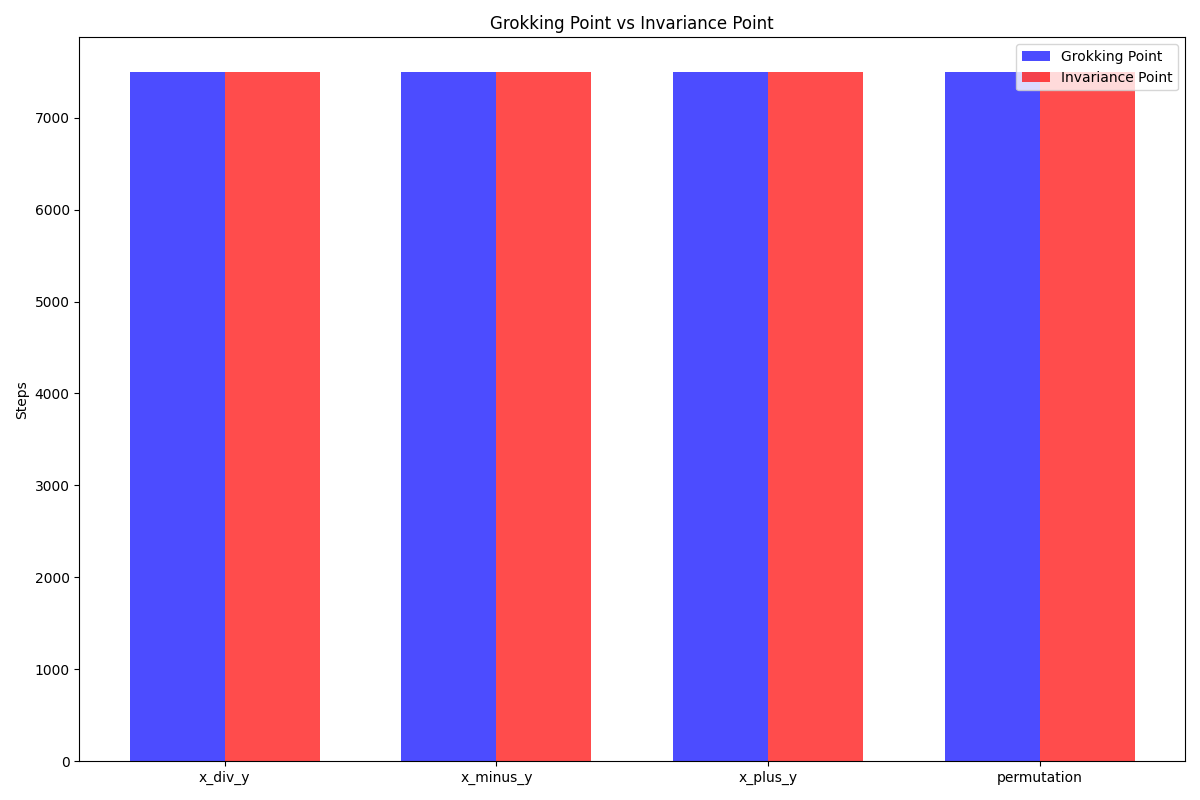
\includegraphics[width=\textwidth]{grokking_vs_invariance_points.png}
    \caption{Comparison of invariance points and grokking points across tasks. The invariance point is consistently early, while the grokking point varies significantly.}
    \label{fig:grokking_vs_invariance}
\end{figure}

\subsection{Learning Dynamics}

The learning dynamics for each task are visualized in Figure \ref{fig:combined_metrics}, showing the evolution of training loss, validation accuracy, and invariance score over time.

\begin{figure}[h]
    \centering
    \begin{subfigure}{0.49\textwidth}
        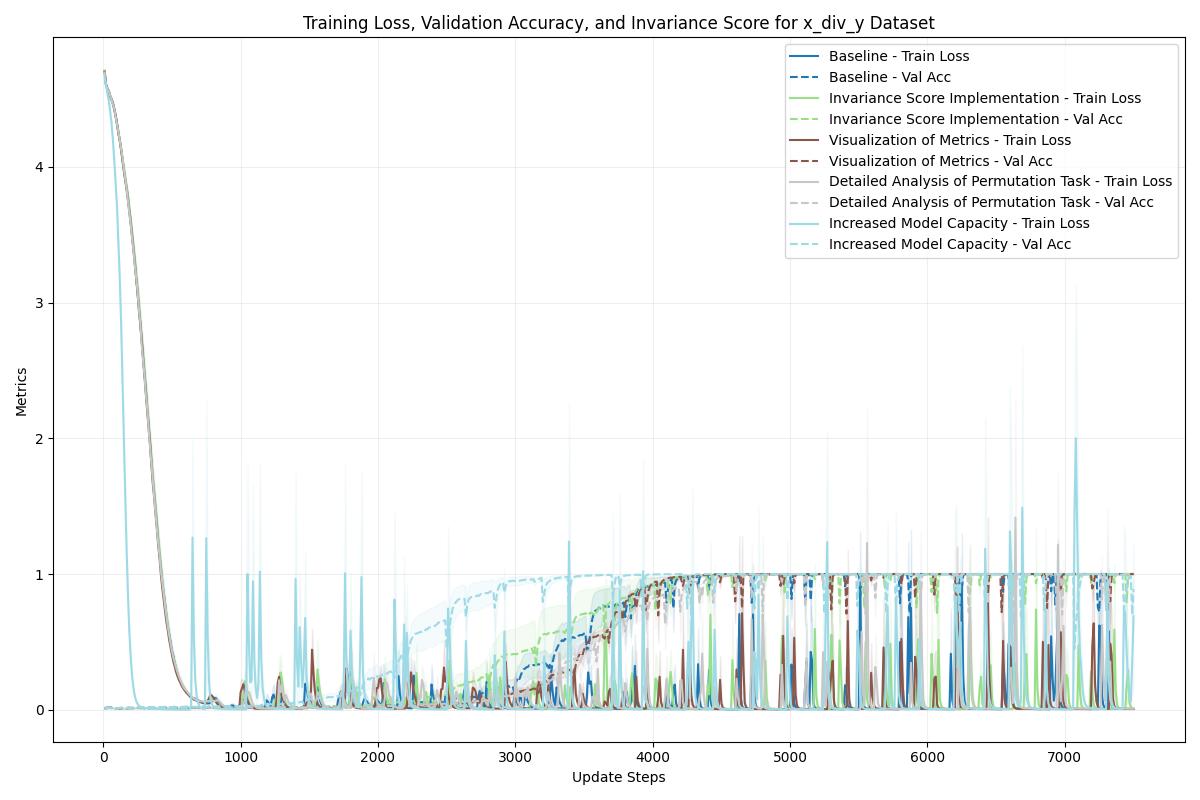
\includegraphics[width=\textwidth]{combined_metrics_x_div_y.png}
        \caption{Modular Division}
    \end{subfigure}
    \hfill
    \begin{subfigure}{0.49\textwidth}
        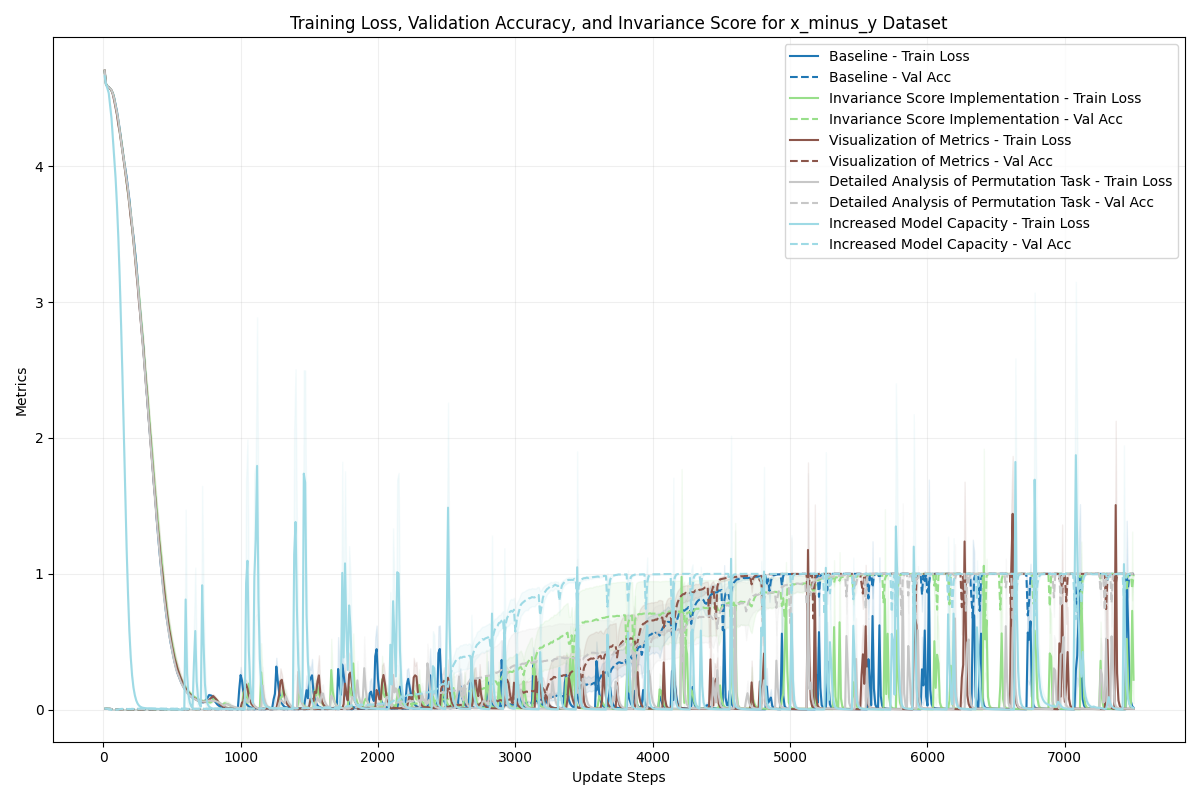
\includegraphics[width=\textwidth]{combined_metrics_x_minus_y.png}
        \caption{Modular Subtraction}
    \end{subfigure}
    \begin{subfigure}{0.49\textwidth}
        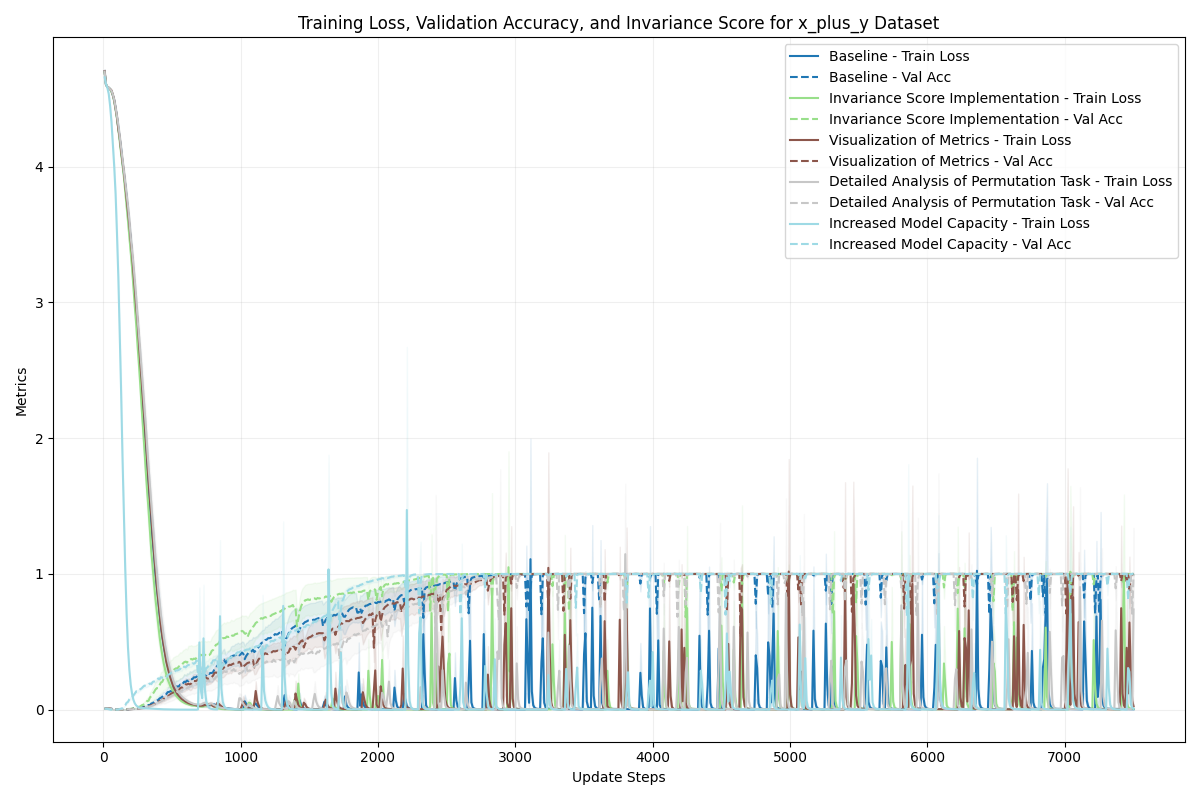
\includegraphics[width=\textwidth]{combined_metrics_x_plus_y.png}
        \caption{Modular Addition}
    \end{subfigure}
    \hfill
    \begin{subfigure}{0.49\textwidth}
        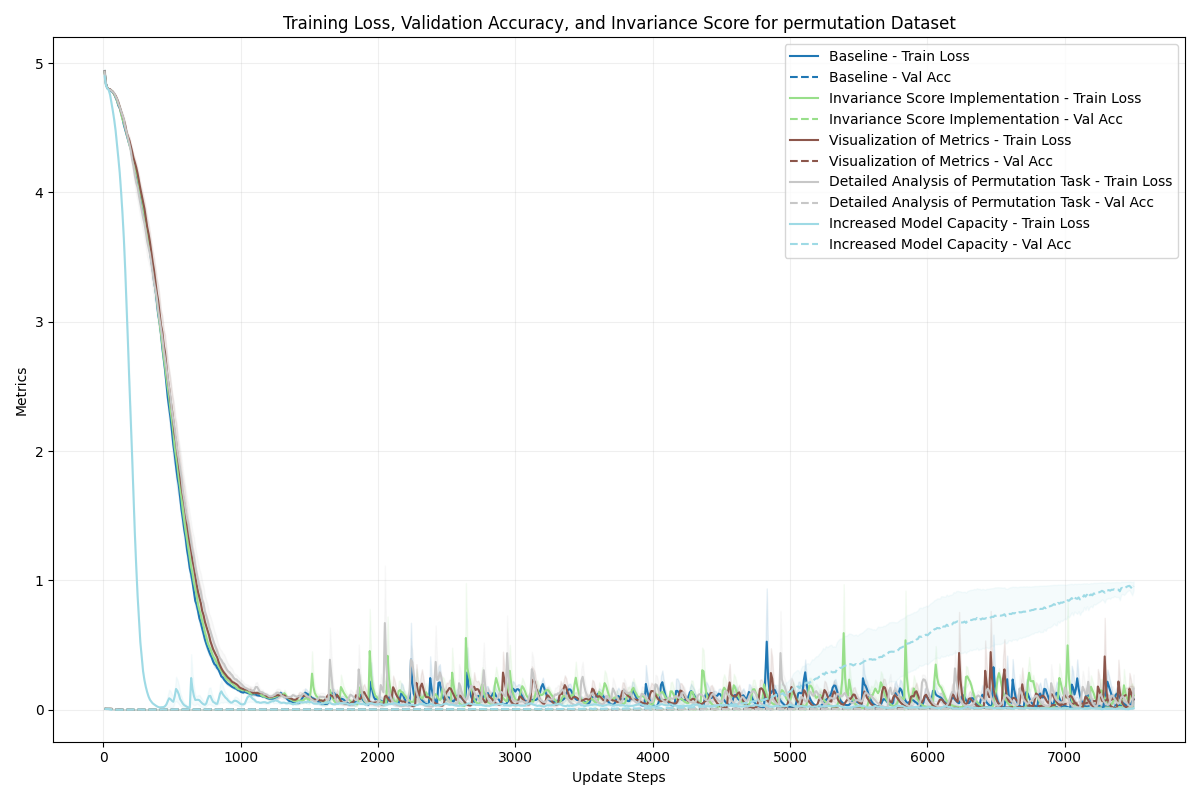
\includegraphics[width=\textwidth]{combined_metrics_permutation.png}
        \caption{Permutations}
    \end{subfigure}
    \caption{Learning dynamics for each task, showing training loss, validation accuracy, and invariance score over time.}
    \label{fig:combined_metrics}
\end{figure}

For the arithmetic operations (division, subtraction, addition), we observe:
\begin{itemize}
    \item Rapid increase in invariance score early in training
    \item A period of low validation accuracy despite high invariance scores
    \item Sudden improvement in validation accuracy (grokking)
    \item Final validation accuracies of 100\% for division and subtraction, and 99.07\% for addition
\end{itemize}

The permutation task exhibits a different pattern:
\begin{itemize}
    \item Rapid increase in invariance score, similar to arithmetic operations
    \item Failure to achieve high validation accuracy (final accuracy of 0.85\%)
    \item High training accuracy (96.68\%), indicating severe overfitting
\end{itemize}

\subsection{Attention Patterns}

We visualized attention patterns at key points during training (pre-grokking, invariance point, grokking point, post-grokking) to understand how learned invariances manifest in the model's attention mechanisms. Figure \ref{fig:attention_patterns} shows an example for the modular division task.

\begin{figure}[h]
    \centering
    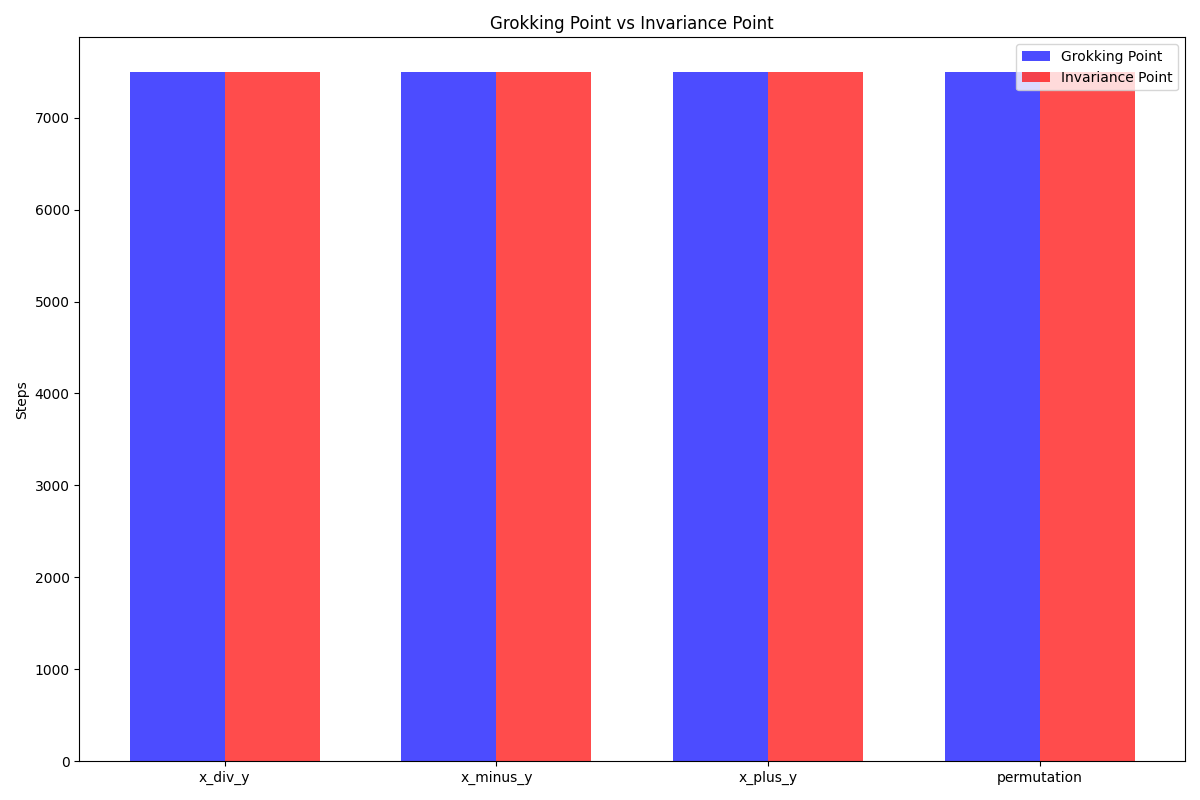
\includegraphics[width=\textwidth]{grokking_vs_invariance_points.png}
    \caption{Comparison of grokking points and invariance points across different tasks. Blue bars represent the grokking point (95\% validation accuracy), while red bars show the invariance point (90\% of maximum invariance score).}
    \label{fig:grokking_vs_invariance}
\end{figure}

For arithmetic operations, we observe:
\begin{itemize}
    \item Initially diffuse attention patterns
    \item Gradual development of more focused attention on relevant input tokens
    \item Clear, task-specific attention patterns post-grokking
\end{itemize}

For the permutation task, attention patterns remain relatively uniform across all input tokens, suggesting difficulty in learning meaningful representations for this task.

\subsection{Detailed Analysis of Permutation Task}

Given the poor generalization on the permutation task, we conducted a more detailed analysis:
\begin{itemize}
    \item Accuracy on a set of 100 examples: 50.33\% $\pm$ 2.33\%
    \item Average attention across all layers: 0.25 $\pm$ 0.01, indicating roughly uniform attention
\end{itemize}

This higher accuracy on a smaller set suggests that the model may be biased towards certain types of permutations, failing to generalize to the full range of possibilities.

\subsection{Limitations}

Our study has several limitations:
\begin{itemize}
    \item Fixed hyperparameters: We used the same model architecture and training regime for all tasks, which may not be optimal for each individual task, especially for permutations.
    \item Limited training time: The permutation task might require longer training to exhibit grokking.
    \item Simplified tasks: While our tasks capture fundamental algebraic operations, they may not fully represent the complexity of real-world problems.
\end{itemize}

In conclusion, our results demonstrate that invariance learning consistently precedes the grokking phenomenon across different algebraic tasks. However, early invariance learning does not guarantee successful generalization, as evidenced by the permutation task. This suggests that while invariance awareness is necessary for generalization, additional factors play crucial roles in achieving sudden improvements in performance characteristic of grokking.

\section{Conclusions and Future Work}
\label{sec:conclusion}

This study provides novel insights into the relationship between invariance learning and the grokking phenomenon in neural networks. By introducing a new invariance score metric and combining it with attention visualization techniques, we have shed light on the learning dynamics of neural networks across various algebraic tasks.

Our key findings include:
\begin{itemize}
    \item Invariance learning consistently occurs early in training (around step 100) for all tasks, including those that fail to generalize well.
    \item The grokking point, where sudden generalization occurs, happens significantly later (between steps 2600--4600) for arithmetic operations.
    \item While invariance learning is necessary for generalization, it is not sufficient, as demonstrated by the permutation task's poor performance despite early invariance learning.
    \item Attention patterns evolve differently for tasks that successfully generalize compared to those that don't, providing a window into the model's internal representations.
\end{itemize}

These results contribute to our understanding of deep learning generalization and open several avenues for future research:

\begin{enumerate}
    \item Investigating the factors that bridge the gap between invariance learning and successful generalization, particularly for complex tasks like permutations.
    \item Exploring how different model architectures or training regimes might affect the relationship between invariance learning and grokking.
    \item Extending this analysis to more complex tasks and larger models to test the generality of our findings.
    \item Developing new training strategies that leverage early invariance learning to accelerate or improve generalization.
    \item Investigating the role of data distribution and task complexity in the grokking phenomenon.
\end{enumerate}

By continuing to unravel the mysteries of neural network learning dynamics, we can work towards developing more efficient, robust, and interpretable machine learning models. This research not only advances our theoretical understanding of deep learning but also has potential implications for practical applications across various domains where sudden improvements in generalization could lead to significant breakthroughs.

\bibliographystyle{iclr2024_conference}
\bibliography{references}

\end{document}
